\documentclass[a4paper, 12pt]{article}

\usepackage[T2A]{fontenc}
\usepackage[utf8]{inputenc}
\usepackage[english,russian]{babel}
\usepackage[left=15mm, top=20mm, right=15mm, bottom=20mm, nohead, nofoot]{geometry}

\usepackage{hyperref}
\usepackage{graphicx}
\usepackage{wrapfig}
\usepackage{afterpage}
\usepackage{amsmath, amsfonts, amssymb, amsthm, mathtools}
\author{Хомутов Андрей, группа Б06-903}
\title{Лабораторная работа 3.1.3 \\ Измерение магнитного поля земли
}
\date{30 сентября 2020 г.}

\begin{document}

\maketitle
\thispagestyle{empty}
\newpage

\section*{Цель работы} 
\textbf{Определить} характеристики шарообразных неодимовых магнитов и, используя законы взаимодействия магнитных моментов с полем, измеритьгоризонтальную и вертикальную составляющие индукции магнитного поля Земли и магнитное наклонение.


\section*{В работе используются}
12 одинаковых неодимовых магнитных шариков, тонкая нить для изготовления крутильного маятника, медная проволока диаметром (0,5 –0,6)мм, электронные весы, секундомер, измеритель магнитной индукции АТЕ-8702,штангенциркуль, брусок из немагнитного материала  (25х30х60  мм3), деревянная  линейка, штативиз  немагнитного  материала;дополнительные неодимовые магнитные шарики (~ 20 шт.) и неодимовые магниты в форме парал-лелепипедов (2 шт.), набор гирь и разновесов.
 
\section{Теоретическая часть}
\subsection{Точечный магнитный диполь}
Простейший магнитный диполь может быть образован витком с током или постоянным магнитом.По определению,магнитный момент $\vec{P}_{m}$ тонкого витка площадью S током $I$ равен:
\begin{equation}\vec{P}_{m}=(I / c) \vec{S}=(I / c) S \vec{n}\end{equation}
где с–скорость света в вакууме,$\vec{S}=S \vec{n}$ - вектор площади контура, образующий с направлением тока правовинтовую систему,  $\vec{n}$—единичный вектор нормали к площадке S(это же направление $\vec{P}_{m}$ принимается за направление S -> N от южного (S) к северному (N) полюсу).Если размеры кон-тура с током или магнитной стрелки малыпо сравнению расстоянием до диполя, то соответствую-щий магнитный диполь $\vec{P}_{m}$ называют элементарным или точечным.

Магнитное поле точечного диполя определяется по формуле, аналогичной формуле для поля элементарногоэлектрического диполя
\begin{equation}\vec{B}=3\left(\vec{P}_{m} \vec{r}\right) \vec{r} / r^{5}-\vec{P}_{m} / r^{3}\end{equation}
В магнитном поле c индукцией B на точечный магнитный диполь действует механический момент сил:
\begin{equation}\vec{M}=\vec{P}_{m} \times \vec{B}\end{equation}
Под действием вращающего момента $\vec{M}$ виток с током или постоянный магнит поворачивается так, чтобы его магнитный момент выстроился вдоль вектора индукции магнитного поля. Это —положение устойчивого равновесия: при отклонении от этого положения возникает механический момент внешних сил, возвращающий диполь к положению равновесия. В положении, когда $\vec{P}_{m}$ и $\vec{B}$ параллельны, но направлены противоположно друг другу, также имеет место равновесие (M=0), но такое равновесие неустойчиво: малейшее отклонение от этого положения приведёт к появлению момента сил, стремящихся отклонить диполь ещё дальше от начального положения.Магнитный диполь в магнитном поле обладает энергией:
\begin{equation}W=-\left(\vec{P}_{m}, \vec{B}\right)\end{equation}
Из этой формулы следует, что энергия диполя в поле минимальнаи равна $W_{\min }=-P_{m} B$ при сонаправленных векторах $\vec{P}_{m} \uparrow \uparrow \vec{B}$ (угол $\theta$ между $\vec{P}_{m}$ и $\vec{B}$ равен нулю), т.е., как и следовало ожидать,в положении устойчивого равновесия.
В неоднородномполе на точечный магнитный диполь, кроме момента сил, действует ещё и сила:
\begin{equation}\vec{F}=(\vec{P}, \vec{\nabla}) \vec{B},\end{equation}
где $\vec{\nabla}=\left(\frac{\partial}{\partial x}, \frac{\partial}{\partial y}, \frac{\partial}{\partial z}\right)$ - дифференциальный оператор Гамильтона(векторный оператор «набла»).

Используя формулы для момента силы, силы и энергии, не сложно выяснить, как ведёт себя свободный магнитный диполь в неоднородном магнитном поле: он выстраивается вдоль силовых линий магнитного поля и, кроме того, под действием результирующей силы, возникающей из-за неоднородности поля,втягивается в область более сильного магнитного поля, т.е. в область, где он обладает меньшей энергией. Зная магнитные моменты $P_{1}$ и $P_{2}$ двух небольших постоянных магнитов, можно рассчитать силу их взаимодействия. Если магнитные моменты $P_{1}=P_{2}=P_{m}$ двух одинаковых небольших магнитов направлены вдоль соединяющей их прямой, а расстояние между ними равно r, то магниты  взаимо-действуют с силой: \begin{equation}F=P_{m} \partial B / \partial r=P_{m} \partial\left(2 P_{m} / r^{3}\right) / \partial r=-6 P_{m}^{2} / r^{4}\end{equation}Магниты притягиваются, если их магнитные моменты сонаправлены $\left(\vec{P}_{1} \uparrow \uparrow \vec{P}_{2}\right)$ и отталкива-ются, если моменты направлены противоположно друг другу $\left(\vec{P}_{1} \uparrow \downarrow \vec{P}_{2}\right)$. 
\subsection{Неодимовые магнитные шары}
В настоящей работе используются неодимовые магниты шарообразной формы. Для нас важно то, что:
\begin{enumerate}
\item шары намагничены однородно
\item вещество, из которого изготовлены магниты,является магнитожёстким материалoм
\end{enumerate}
Магнитное поле однородно намагниченного шарарадиуса R на расстояниях r ≥ Rот центра шарасовпадает с полем точечного магнитного диполя Pm, равного полному магнитному моменту шараи расположенногов его центре.(Можно показать, что внутри (r < R) такого шара поле однородно и равно $B_{0}=2 P_{m} / R^{3}$).

Магнитожёсткость материала означает, что магнитные моменты шаров в нашей работе не изме-няются под действием внешних магнитных полей, т.е.шар ведёт как жёсткий диполь. Поэтому, при расчетах можно считать, что шары взаимодействуют как жёсткие точечные магнитные диполи, рас-положенные в центрах шаров.

Полный магнитный момент mPпостоянного магнита определяется намагниченностью mpвеще-ства, из которого он изготовлен. По определению, намагниченность –это магнитный момент еди-ницы объёма. Для однородно намагниченного шара намагниченность, очевидно,равна:
\begin{equation}\vec{p}_{m}=\vec{P}_{m} / V\end{equation}
где V—объём шара.

Намагниченность —важная характеристика вещества постоянных магнитов, определяющая, в частности, величину остаточной магнитной индукции $B_{r}=4 \pi p_{m}$ (остаточная индукция Вr—одна из величин, которая, как правило, указывается в справочниках по магнитожёстким материалам).Не сложно показать, что индукция магнитного поля Bp на полюсах однородно намагниченного шара связанас величиной намагниченности Рm  и остаточной магнитной индукцией Br формулой:
\begin{equation}\vec{B}_{p}=(8 \pi / 3) \vec{p}_{m}=(2 / 3) \vec{B}_{r}\end{equation}

%\subsection{Экспериментальная установка}


\section{Практическая часть}
\subsection{Снятие и обработка экспериментальных данных}
\subsubsection{Определение магнитного момента,намагниченности и остаточной магнитной индукции вещества магнитных шариков}
\textbf{Метод А:}
\begin{enumerate}
    \item Сначала были измерены масса и диаметр шариков:
    \begin{center}
    $m=0,8495 \pm 0,0001 \: \text{г}, \; r = 0,285 \pm 0,002 \: \text{см}$    
    \end{center}
    \item Подкладывая между шарами немагнитный материал (дерево и бумагу) было измерено макисмальное расстояние $r_{max} = 2,78  \pm 0,01 \: \text{см}$, на котором один шарик способен удержать другой в поле тяжести Земли. Чрезвычайно важен тот факт, что формулы для расчета были выведены в СГС, а потому дальнейшие значения магнитных величин выражаются в соответсвующих единицах измерения (сантиметр-грамм-секунда) и лишь в конце величина магнитного поля будет предоставлена в еденицах СИ.
    \begin{figure}[h]
    \begin{center}
    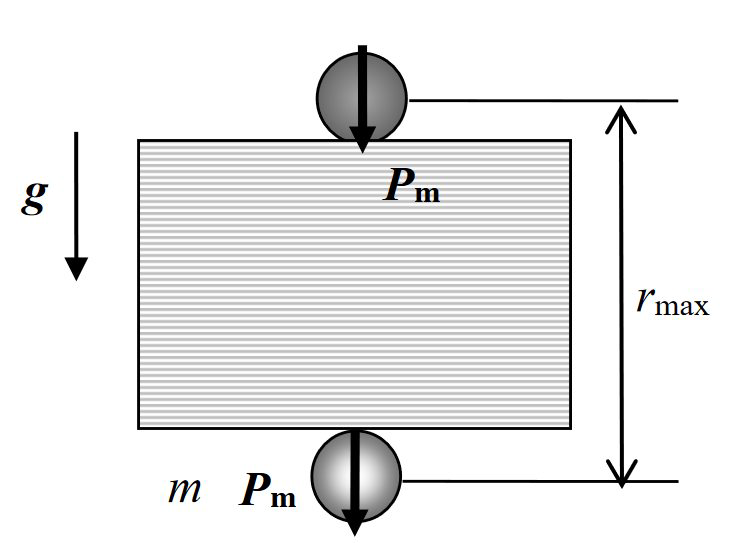
\includegraphics[width=0.5\textwidth]{метод А.png}
    \end{center}
    \caption{Метод А}
    \end{figure}
    \item Зная, что $F=6 P_{m}^{2} / r_{\max }^{4}$, а  $F_{T} = mg$, мы можем расчитать расчитать магнитный момент шариков:
    \begin{displaymath} P_{m}=r_{m}^{2} \sqrt{\frac{m g}{6}} = (91,1 \pm 1,6)  \frac{\text{г}^{\frac{1}{2}} \text{cм}^{\frac{5}{2}}}{c}\end{displaymath}
    При этом погрешность расчета магнитного моменоа оценивалась как:
    \begin{displaymath} \delta_{P_{m}}=\operatorname{Pm}\left(2 \varepsilon_{r}+\frac{1}{2} \varepsilon_{m}\right) \end{displaymath}
    \item По формуле (7) можно рассчитать величину намагнченности шарика $p_{m} = 940 \frac{\text{кг}^{\frac{1}{2}} \text{м}^{\frac{-1}{2}}}{c}$
    \item По формуле (2) мы можем рассчитать величину магнитной индукции на полюсах  $B_{p} = 7870 \; \text{Гс} = 787 \; \text{мТл}$. Имелась возможность эту же величину определить с помощью магнитометра. От измерения к измерению величина магнитного поля на полюсах различалась, она находилась в грамницах от 210 до 335 мТл. Однако точность измерения подтверждает совпадение величины остаточной магнитной индукции с табличными значениями.
    \item Величина остаточной намагниченности получилась равной $B_{r}= (3 / 2) B_{p} = 11805 \text{Гс}$. Табличные значения \footnote{https://ferrite.ru/products/magnets/ndfeb} варьируются от 11 до 13 кГс.
\end{enumerate}

\textbf{Метод Б:}
\begin{wrapfigure}{r}{2cm}
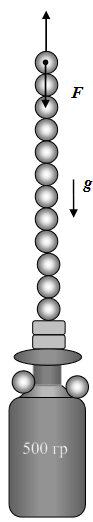
\includegraphics[width=1cm]{Метод Б.png}
\caption{Метод Б}
\end{wrapfigure}
\begin{enumerate}
    \item Используя другую схему, мы можем составить цепь из шаров, подвешивая их друг за друга и добавив груз снизу. По величине силы, при которой происходит отрыв цепи от верхнего шара, можно рассчитать его магнитный момент (рис. 2).
    \item Аналогично методу А можно расчитать дипольный момент шарика по весу оторвавшейся цепочки с грузом. Разница в том что нужно учитывать взаимодействие нескольких шариков друг с другом, а погргешность измерения оторвавшейся массы можно не учитывать (270,97г >> 0,01г):
    \begin{displaymath} P_{m}=d^{2} \sqrt{\frac{F}{6 \cdot 1,08}} = (65,8 \pm 0,3)  \frac{\text{г}^{\frac{1}{2}} \text{cм}^{\frac{5}{2}}}{c}  \end{displaymath}
    \item Аналогично, поле на полюсах шарика  $B_{p} = 5680 \; \text{Гс} = 568\; \text{мТл}$. Непосредственное измерение магнитометром показывает, что измерение, проведенное методом А оказалось точнее.
\end{enumerate}
\subsection{Определение вертикальной составляющей магнитного поля Земли}
Был собран крутильный маятник из n (=3-12) магнитных шариков, после чего измерялся период его колебаний. Погрешность считалась как $\sigma_{T}=\sqrt{\sigma_{\text{случ}}^{2}+\sigma_{\text{реакц}}^{2}}$. Для уменьшения вклада случайной погрешности было проведено 3 измерения периода для каждого n, а для уменьшения вклада систематической одним измерением считалось время которое требовалось весам на совершение не одного, но нескольких (>5) колебаний. Соответсвующие измерения приведены в таблице 1.
\begin{table}[h]
\begin{center}
\caption{T(n)}
\begin{tabular}{|c|c|c|c|c|c|c|}
\hline
n  & К-й & t1, c    & t2, c    & t3, c    & T, c    & \sigma_{T}, c   \\ \hline
12 & 5   & 11,79 & 11,56 & 11,57 & 2,33 & 0,04 \\ \cline{1-1}
11 & 5   & 10,16 & 10,45 & 10,38 & 2,07 & 0,04 \\ \cline{1-1}
10 & 5   & 9,47  & 9,58  & 9,54  & 1,91 & 0,03 \\ \cline{1-1}
9  & 5   & 8,74  & 8,71  & 8,66  & 1,74 & 0,03 \\ \cline{1-1}
8  & 6   & 9,38  & 9,25  & 9,1   & 1,54 & 0,03 \\ \cline{1-1}
7  & 7   & 9,42  & 9,44  & 9,31  & 1,34 & 0,02 \\ \cline{1-1}
6  & 8   & 9,27  & 9,44  & 9,39  & 1,17 & 0,02 \\ \cline{1-1}
5  & 10  & 9,65  & 9,49  & 9,39  & 0,95 & 0,02 \\ \cline{1-1}
4  & 14  & 10,73 & 10,89 & 10,78 & 0,77 & 0,01 \\ \cline{1-1}
3  & 15  & 8,9   & 8,37  & 8,59  & 0,57 & 0,02 \\ \hline
\end{tabular}
\end{center}
\end{table}
\newpage
По данной зависимости был построен график зависимости T(n) и найден коэффициент наклона $k = 0,19$, см рис. 3.
\begin{figure}
    \begin{center}
    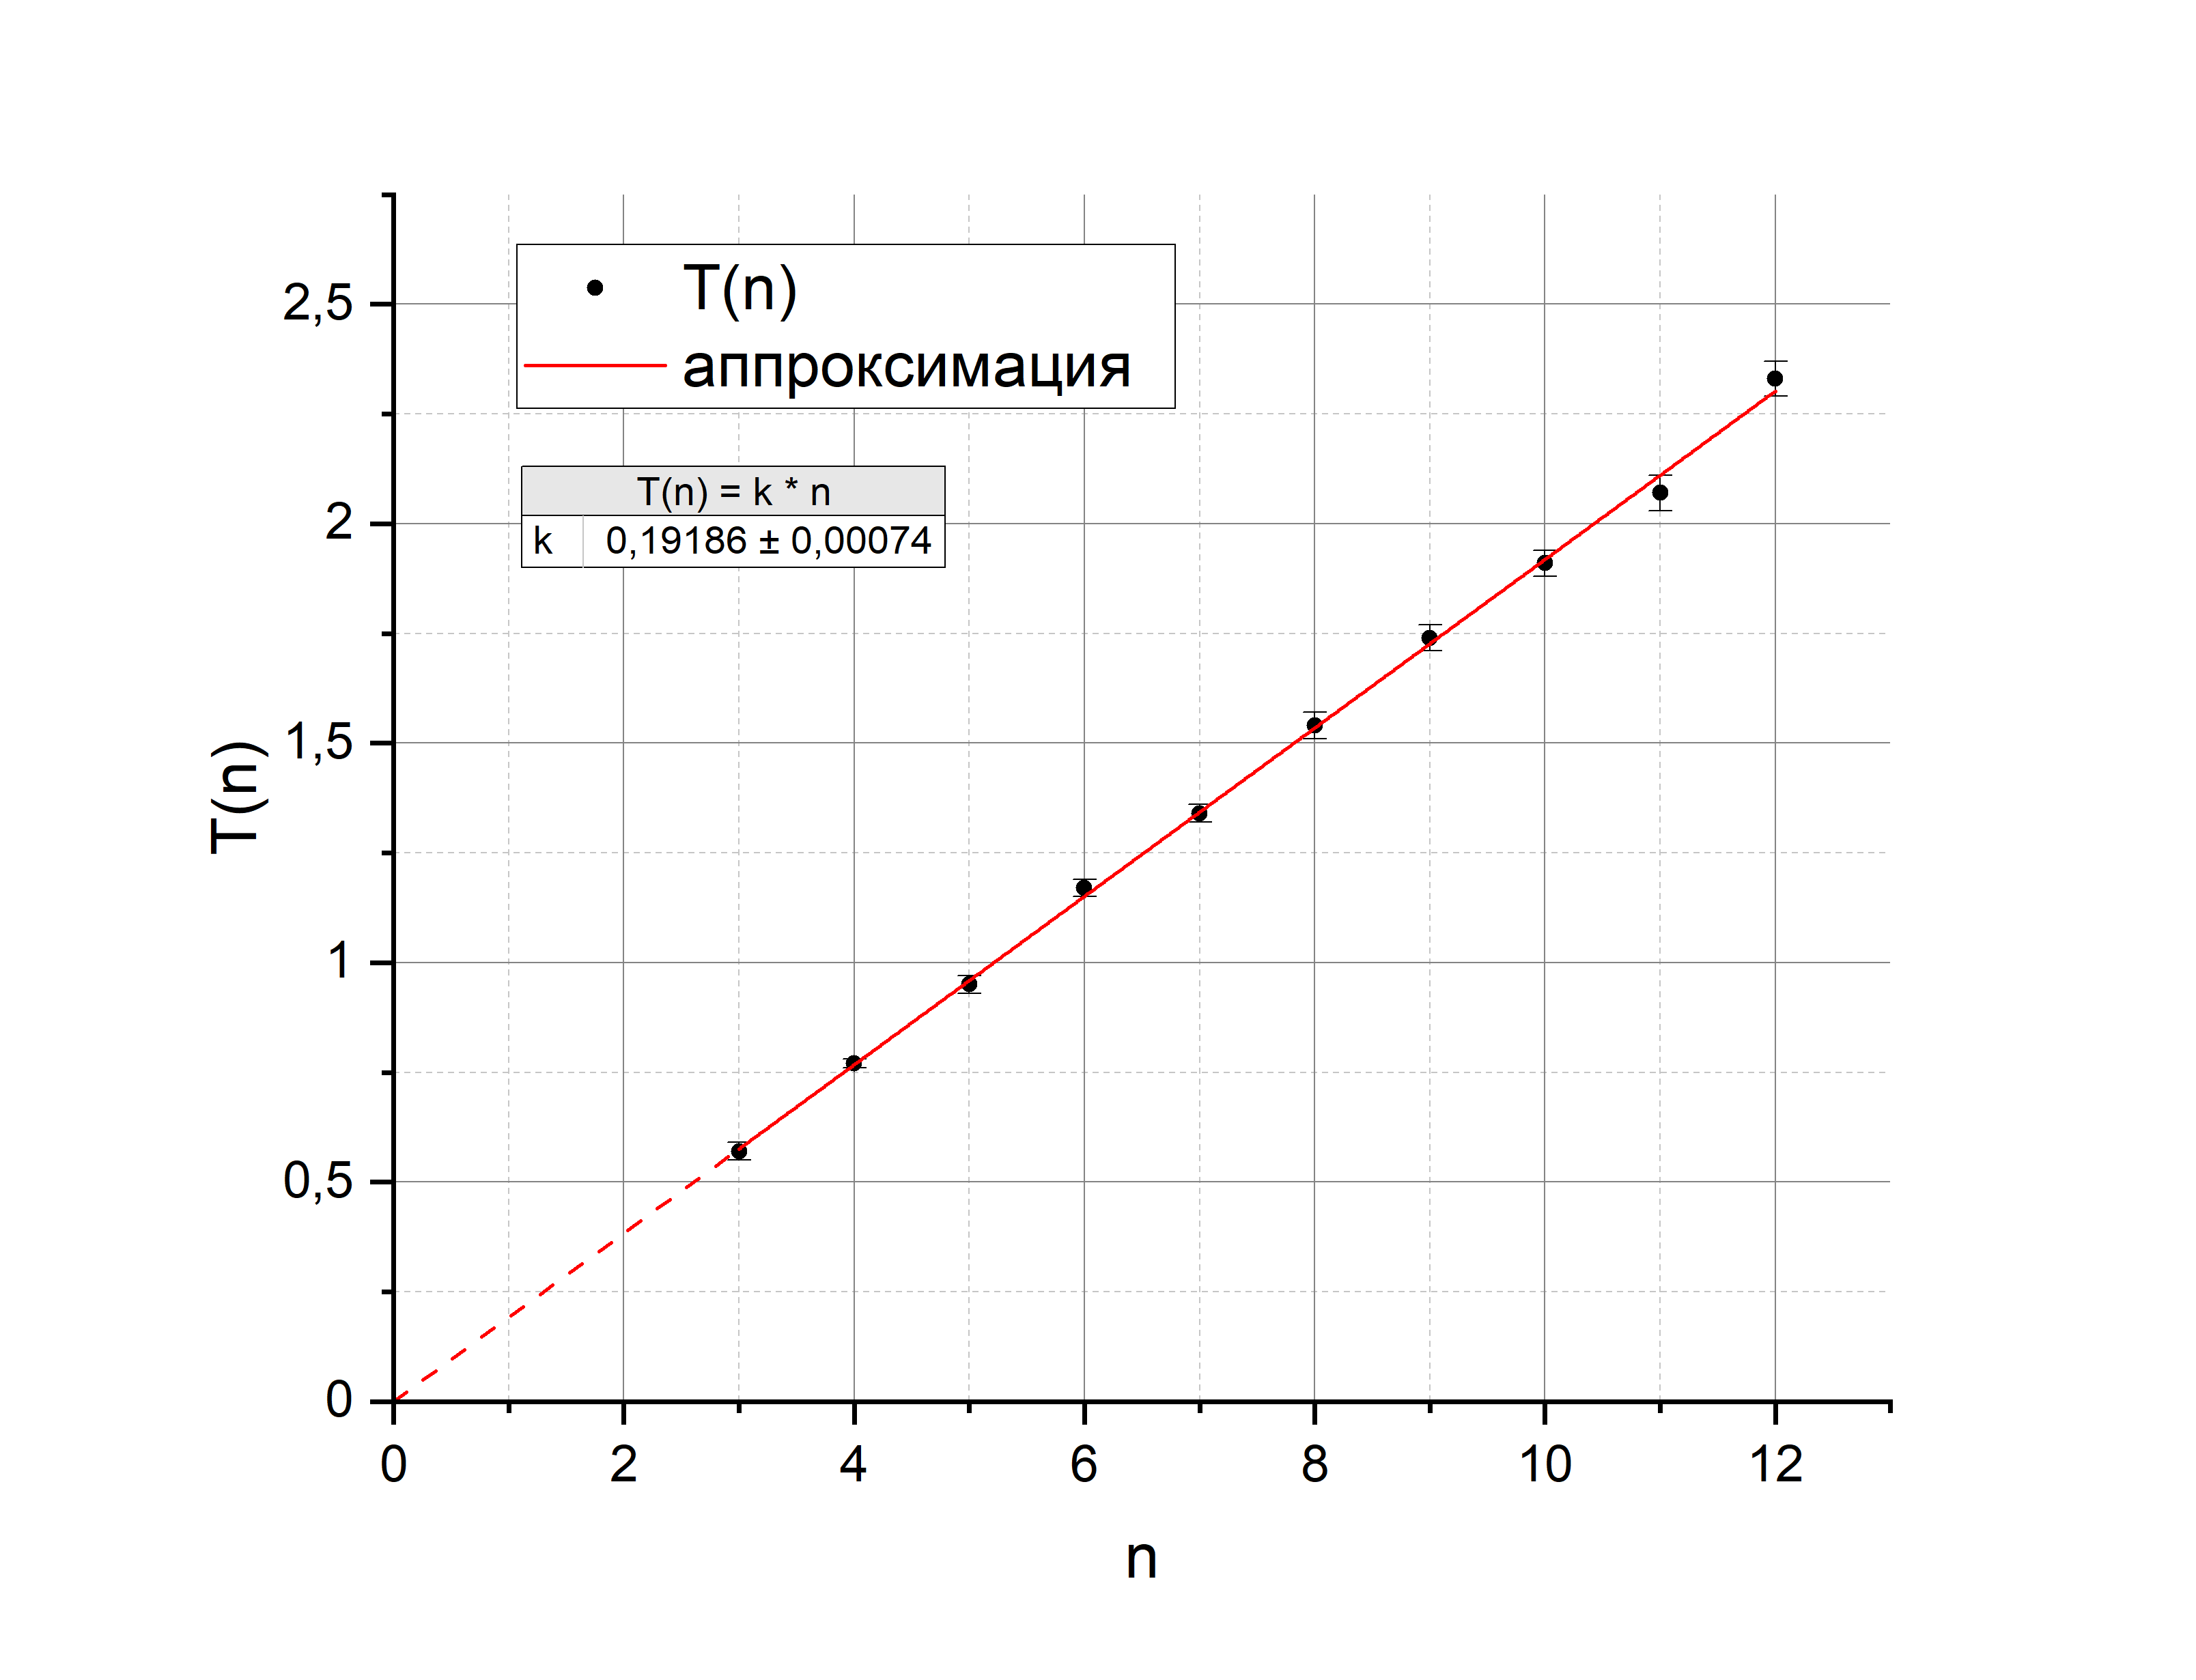
\includegraphics[width=0.7\textwidth]{T(n).png}
    \end{center}
    \caption{T(n)}
    \end{figure}
Cчитая что стержни подчиняются уравнению малых вращательных колебаний, где момент инерции системы шаров совпадает с хорошей точностью с моментом инерции стержня, можно получить:
\begin{equation}B_{h}=\pi^{2} m d^{2} / 3 k^{2} P_{m}\end{equation}
\begin{displaymath} B_{h}= 270 \pm 9 \; \text{мГс,} \end{displaymath}
погрешность рассчитывалась по формуле $\varepsilon_{B_{h}}=\varepsilon_{m}+2 \varepsilon_{d}+2 \varepsilon_{k}+\varepsilon_{P_{m}}$
Если свернуть систему из шариков в кольцо (для которого, очевидно, суммарный дипольныц момент равен нулю), то колебания вообще не наблюдаются, что подтверждает отсутсвие необходимости учитывать собственную упругость нити.
\subsection{Определение вертикальной составляющей магнитного поля Земли}
Была собрана стрелка из четного числа шаров n (=2-10) для которой были измерены величины моментов М, переводивших ее из наклоненного в горизонтальное положение. Этот момент равен величине момента сил, создаваемого вертикальной составляющей магнитного поля Земли. Аналогично зависимости М(n) и график М=А(n) представлены в таблице 2 и на рис. 4.
\begin{table}[h!]
\begin{center}
\caption{M(n)}
\begin{tabular}{|c|c|c|c|c|}
\hline
шариков, n & Плечо, d & m, мгр & M, дин*см & $\delta_{m}$, дин*см \\ \hline
12         & 5        & 118    & 330       & 6  \\
10         & 4        & 123    & 275       & 5  \\
8          & 3        & 129    & 216       & 4  \\
6          & 2        & 150    & 168       & 3  \\
4          & 1        & 204    & 114       & 2  \\ \hline
\end{tabular}
\end{center}
\end{table}
\begin{figure}
    \begin{center}
    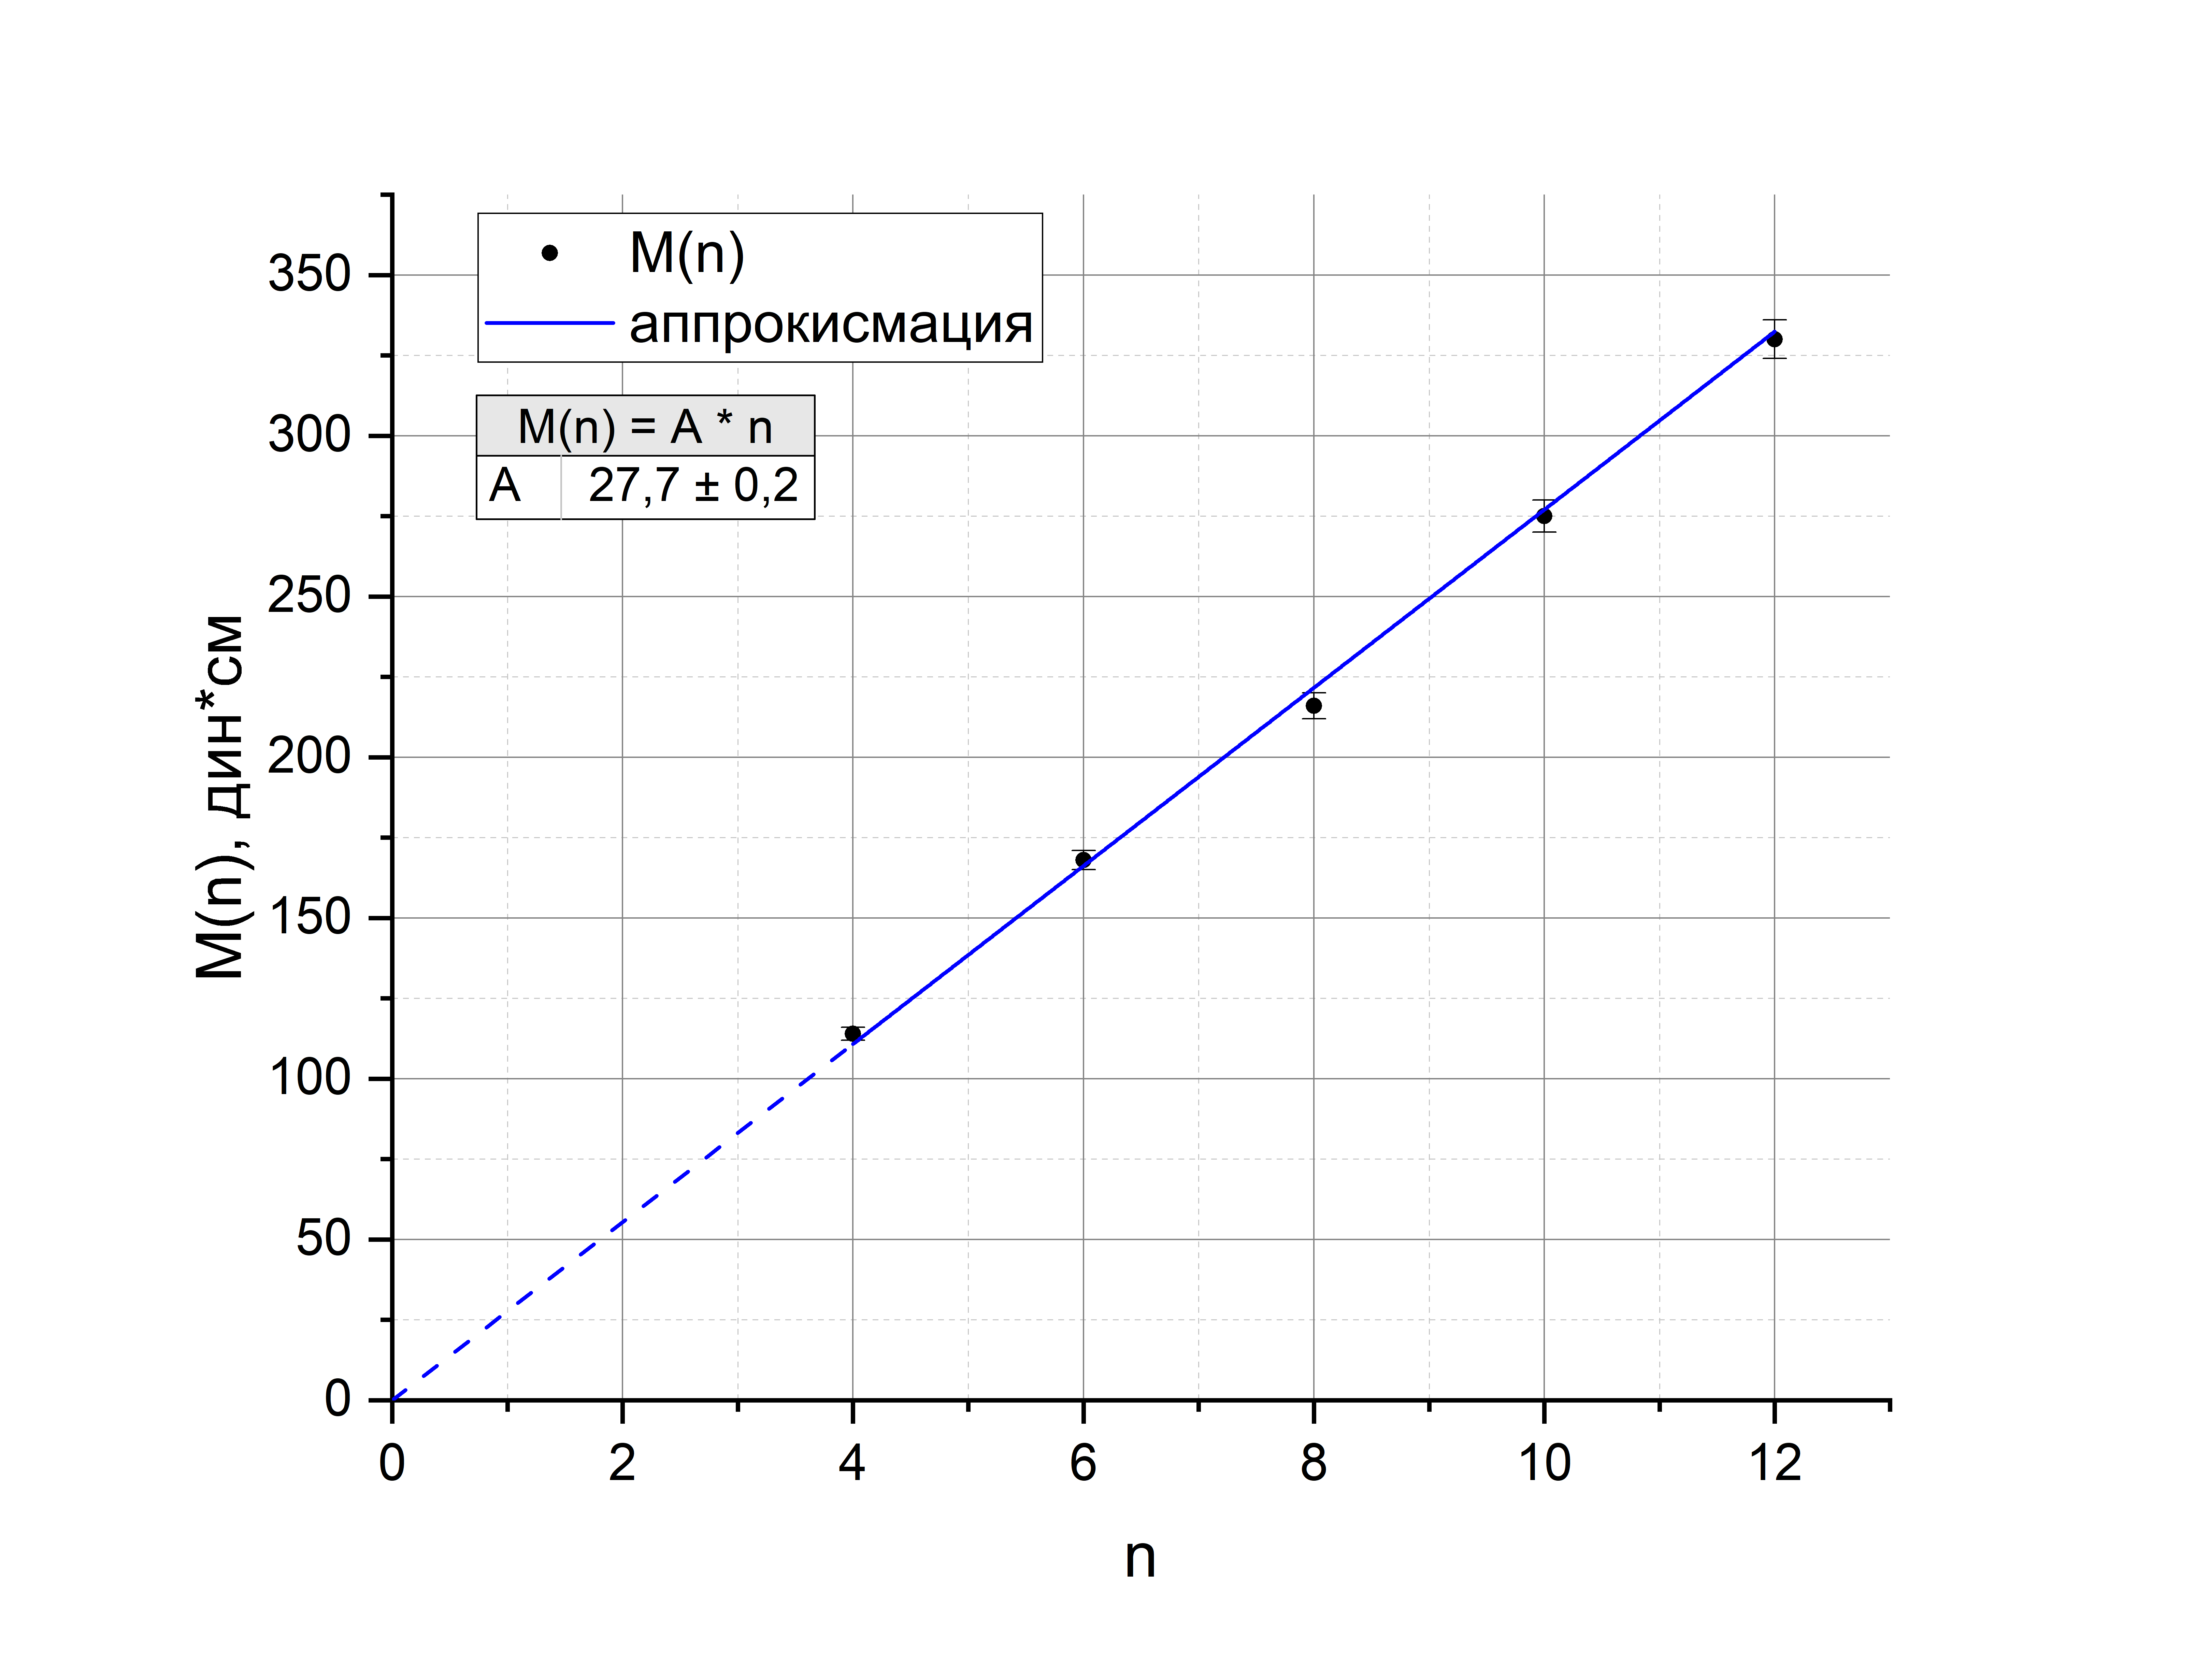
\includegraphics[width=0.7\textwidth]{M(n).png}
    \end{center}
    \caption{M(n)}
    \end{figure}
В силу аддитивности момента сил для n шаров, можно рассчитать вертикальную составляющую как:
\begin{displaymath}B_{v}=A / P_{m} = 304 \pm 07 \; \text{мГс}\end{displaymath}
Теперь мы можем найти магнитное наклонение в месте измерения:
\begin{displaymath} \beta = arctg(B_{v} / B_{h}) = 48,3^{o}\end{displaymath}
Из формулы (2) можно показать, что в модели земли как идеального равномерно намагниченного шара (без учета сдвига дипольного момента относительно центра Земли и наклона относительно оси вращения Земли, равного $11,5^{o}$)  магнитное наклонение на широте $\varphi = 56^{o}$C равнялось бы:
\begin{displaymath} \beta=\operatorname{arctg}\left(\frac{2 \cos \varphi}{\sin \varphi}\right) = 53,5^{o} \end{displaymath}
В рамках этой модели можно рассчитать магнитный момент Земли:
    \begin{equation}
    B_{v}=\frac{2\left(\bar{P}_{m} \cdot \bar{R}\right)}{R^{4}} \Rightarrow P_{m}=\frac{1}{2} \frac{B_{v} \cdot R^{3}}{\cos \varphi} \end{equation}
    \begin{displaymath} P_{m}= 1,16 \cdot 10^{18} \text{A} \cdot \text{м}^{2}\end{displaymath}
    Точные значения магнитных величин, которые удалось найти:
    \begin{displaymath} B_{h}^{\, ecv}= 300\; \text{мГс,} \;  B_{v}^{\, pol}= 600 \; \text{мГс}\end{displaymath}
    \begin{displaymath} \beta = 71,7^{o}, \; P_{m} \simeq 8 \cdot 10^{22} \text{A} \cdot \text{м}^{2}  \end{displaymath}
    


%\subsection{Обработка результатов измерений}

 \section{Выводы}
\begin{enumerate}
    \item Определение дипольного момента с помощью двух различных методов дало существенно различающиеся результаты. Однако в пользу метода А играет тот факт, что рассчитанная по дипольному моменту величина остаточной магнитной индукуии совпадает с табличными значениями для сплавов Ne-Fe-B. Существенное значение в величине можно объяснить малой точностью эксперимента. Граничная масса при которой верхний шарик отрывался была слабо различима, так как мы были ограничены в выборе грузов. Для матода А мы были способны подобрать граничное расстояние, подкладывая необходимое количество листов.
    \item Была исследована зависимость периода крутильных колебаний стрелки, составленной из магнитных шариков, от количества шариков в стрелке. Зависимость с убедительной точностью вышла линейной, что позволило определить значение Bh с низкой относительной погрешностью. Упругость нити действительно не было ноебхожимо учитывать, в чем можно было убедиться, удостоверившись в отсутсвии колебаний кольца, составленного из шариков.
    \item Аналогично была получена линейная зависимость момента сил уравновешивающего стрелку, от количества шариков в стрелке. Отмечу, что может юыть неучтена погрешность определения горизонтального положения стрелки экспериментатором.
    \item По полученным значениям имелась возможность определить магнитное наклонение в географической точке эксперимента. Оно получилось равным около 53 градусов, что визуально совпадает с наблюдаемым отклонением. Отличие от реальной его величины объясняется допущением в модели, что магнитные полюса Земли совпадают с географическими (вкупе с фактом что центр диполя эквивалентно представляющего магнитное поле земли сдвинут относительно ее геометрического центра). Однако по порядку величины значения магнитной индукции укладываются в диапазон, накладываемый вертикольной составляющей В на полюсе и горизонатльной на экваторе.
    \item Также модель абсолютно непригодна для определения магнитного момента Земли, если верить найденным табличным значением, различие с которым составляет несколько порядков.

\end{enumerate}


\end{document}

